\section{Relative work}
Our existing snake-liked robot platform is shown in~\figref{fig:snake_like_robot_a}. The joints of snake-liked robots are connected orthogonally. We also build the simulation snake-liked robot(~\figref{fig:snake_like_robot_b}) and embeded a set of sensors like angle sensors and distance sensors to realize the feedback control of robots.
\begin{figure}[!t]
	\centering
	\subfigure[Reality robot]{
		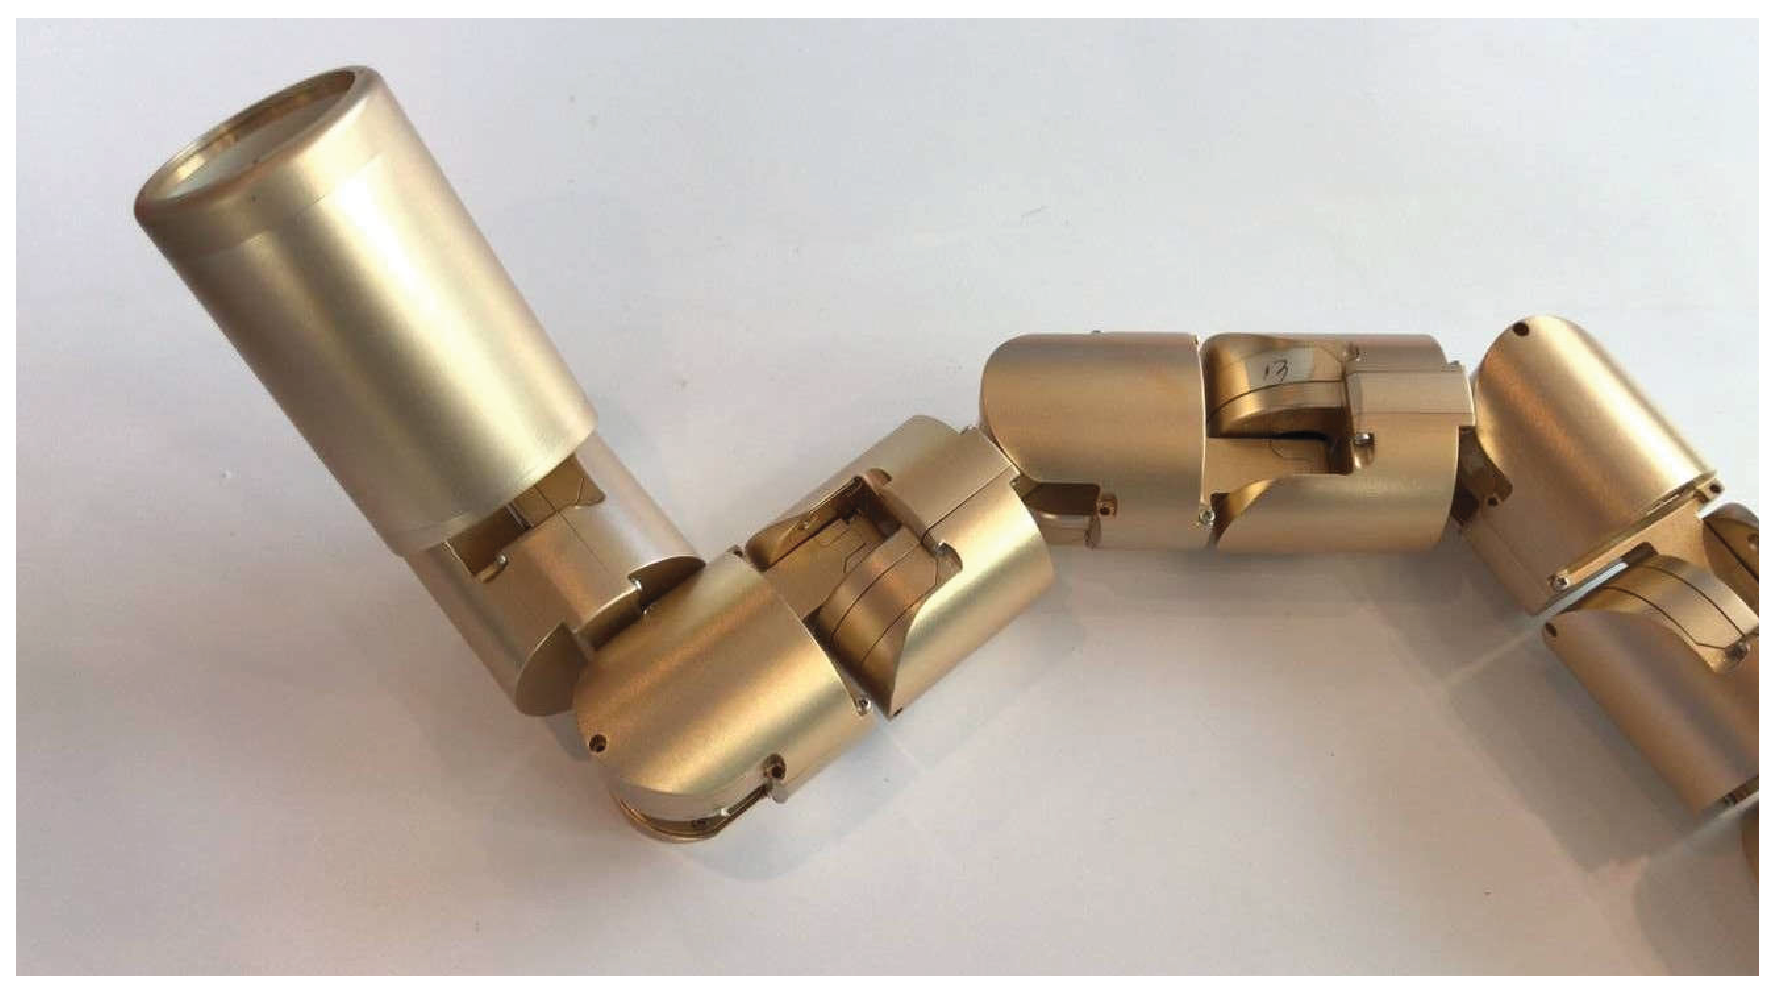
\includegraphics[width=1.5in,height=0.75in]{fig/relative/realSnake}
		\figlabel{fig:snake_like_robot_a}
	}
	\subfigure[Simulation robot]{
		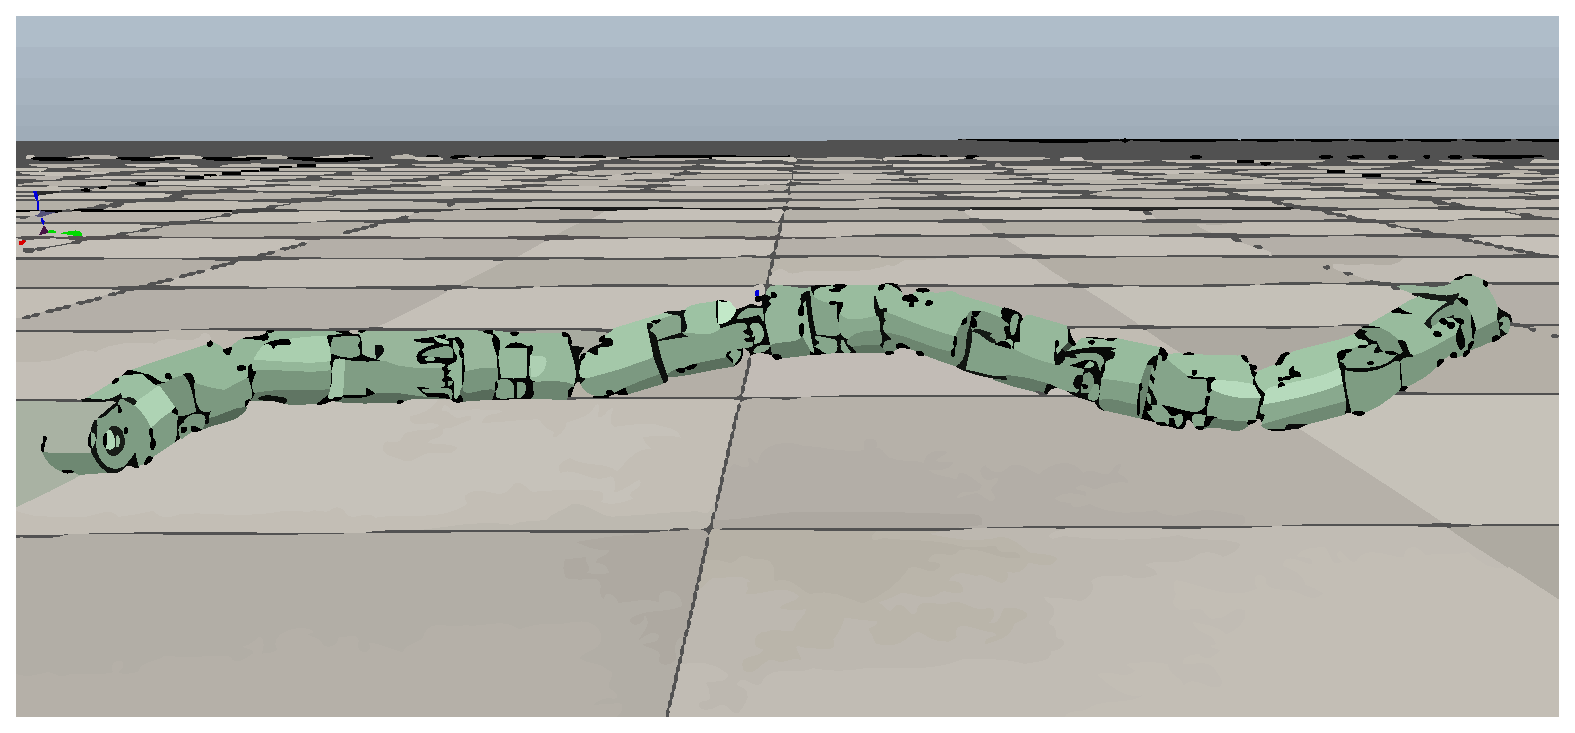
\includegraphics[width=1.5in,height=0.75in]{fig/relative/simulateSnake}
		\figlabel{fig:snake_like_robot_b}
	}
	\caption{The Snake-liked robot}
	\figlabel{fig:snake_like_robot}
\end{figure}

Currently, a widely used of control strategy for snake-liked robots is based on the sinusoidal motion model\cite{HiroseSine} which is proposed by professor Hirose. After that, Tesch et al. proposed a parametric equation based on the sinusoidal model for a snake-liked robot with three-dimensional athleticism\cite{ChosetSine}. This parametric equation simplifies the control strategy of the snake-like robots and allows the robot to determine the movement model of the machine with a small amount of control parameters. In order to ensure that snake-like robots can be applied to a wider scene, robots need to have autonomous mobility in the unknown and complex environment. Therefore, we propose a control strategy by experience-based learning combined with clustering~\cite{Cluseter_ICT,KmeansAndDeepLearning} and weighted regression.

%To make the robots adapt to the unknown environment, the method which use the sensors to perceive the environment and embed the environment perception rules, has been widely used\cite{CPGenabling}\cite{GaitBasedCompliant}\cite{BalancingAndControl}\cite{FeedbackControlOfSoft}. Tang et al. proposed a control strategy based on CPG(central pattern generator) model\cite{CPGenabling}. Rollinson et al. proposed a snake-like robot adaptive control based on state estimation\cite{GaitBasedCompliant}. However, a complete correlation prediction model of control parameters is not given in their paper. As their methods is a gradient model based on state estimation, thus they are not suited to the mutation environment. What's more, there are researchers that have proposed a neural network model combined with physical environment information to determine the control scheme\cite{InformationDriven}\cite{NovelPlasticityRule}\cite{MissileSystems}\cite{NeuroFuzzyBayesian}. This model is only the control suggestion and may not make a good effect on motion in real-time motion of the robot. 
%To make the robots adapt to the unknown environment, the method which use the sensors to perceive the environment and embed the environment perception rules, has been widely used\cite{CPGenabling}\cite{GaitBasedCompliant}\cite{BalancingAndControl}\cite{FeedbackControlOfSoft}. Tang et al. proposed a control strategy based on CPG(central pattern generator) model\cite{CPGenabling}. Rollinson et al. proposed a snake-like robot adaptive control based on state estimation\cite{GaitBasedCompliant}. However, a complete correlation prediction model of control parameters is not given in their paper. As their methods is a gradient model based on state estimation, they are not suited to the mutation environment.
%To adapt to the environment, the method which use the sensors to perceive the environment and embed the environment perception rules, has been widely used\cite{CPGenabling}\cite{GaitBasedCompliant}\cite{BalancingAndControl}\cite{FeedbackControlOfSoft}. Tang et al. proposed a control strategy based on CPG(central pattern generator) model\cite{CPGenabling}. They achieve to control the gait change to adapt to the environment by taking speed as a measure,  embedding several gaits to the robots and combining with CPG control according to the environment. Rollinson et al. proposed a snake-like robot adaptive control based on state estimation\cite{GaitBasedCompliant}. A complete correlation prediction model of control parameters is not given in their paper. As it is based on state estimation, this method is a step-by-step change model, thus it is not suited to the mutation environment. %There are some algorithms of machine learning in the robot control applications\cite{InformationDriven}\cite{NovelPlasticityRule}\cite{MissileSystems}\cite{NeuroFuzzyBayesian}. They only give control program conversion but do not provide changes in the control strategy.

%On the application of machine learning in the field of robot control, there are researchers that have proposed a neural network model combined with physical environment information to determine the control scheme\cite{InformationDriven}\cite{NovelPlasticityRule}\cite{MissileSystems}\cite{NeuroFuzzyBayesian}. This model is only the control suggestion and may not make a good effect on motion in real-time motion of the robot. 

%In this paper, a control strategy by experience-based learning  is proposed. Combined with the clustering\cite{Cluseter_ICT}\cite{KmeansAndDeepLearning} and the multi-parameter regression, we realize the real-time autonomous change of multiple control parameters in the robots' movement.
